\documentclass[12pt]{article}
\usepackage[margin=1in]{geometry}
\usepackage{enumitem}
\usepackage{titlesec}
\usepackage{parskip}
\usepackage{graphicx}
\usepackage{hyperref}
\usepackage{fontenc}
\usepackage{amsmath}
\usepackage{xcolor}

\title{\textbf{Lijphart 1999 RG Notes}\\
\large Lijphart, Arend. \textit{Patterns of Democracy: Government Forms and Performance in Thirty-Six Countries}.\\
New Haven: Yale University Press, 1999.}
\author{}
\date{}

\begin{document}

\maketitle

\section{Main Idea}



%--------------------------------------------------
\section{General Notes}
%--------------------------------------------------

\begin{itemize}[leftmargin=*, itemsep=4pt]
    \item Primary breakdown of majoritarian versus consensual government: government \emph{by} the people (representation in office-holding) versus government \emph{for} the people (reflection of representation in policymaking). Majoritarianism seeks to benefit the majority as explicitly as possible; consensus model seeks to include \emph{as many people as possible}. Exclusive/adversarial vs. inclusive/compromising; Kaiser 1997 terms it ``negotiation democracy''
    \item Two dimensions of democratic characterization:
    \begin{itemize}
        \item Executives-parties dimension
        \begin{enumerate}
            \item \underline{Concentration of executive power in single-party cabinets}
            \begin{itemize}
                \item Lowell's (1896) axiom posits that coalition cabinets are much weaker and less stable than single-party cabinets: ``The larger the number of discordant groups that form the majority, the harder the task of pleasing them all, and the more feeble and unstable the position of the cabinet.''
                \item Most appropriate metric of \# of parties seems to be the ``effective number of parties,'' calculated as 
                \begin{align*}
                    N &= \frac{1}{\sum s_i^2}
                \end{align*}
                where $s_i$ is the proportion of seats held by the $i$th party. Depends not only on number of parties, but on their shared relative strength: if heavily imbalanced, $N$ will decrease. Yet, this does not fully account for alliances / coalitions, whereby there may be some -- but not complete -- alignment between parties represented by different vote shares
                \item Dispersion of parties can be highlighted amongst seven issue dimensions:
                \begin{enumerate}
                    \item Socioeconomic
                    \item Religious
                    \item Cultural-ethnic
                    \item Urban-rural
                    \begin{itemize}
                        \item General shift in agrarian parties to enhance appeal towards suburban and rural voters as well, particularly as urbanization has decreased their voting share
                    \end{itemize}
                    \item Regime support
                    \item Foreign policy
                    \item Postmaterialist issues
                \end{enumerate} 
                However, not every democratic system is sensitive to each dimension, and in fact there is some range here: Lijphart characterizes Finland as embodying 3.5 dimensions (counting moderate engagement as one half), while Barbados has only 0.5 dimensions. Still, decently standardized range (not huge variance here). Potentially indicative of an ``exhaustion'' issue, whereby voters can truly only hold so many opinions? Or is this the result of party consolidation such that parties can't effective embody more than a handful of these dimensions without becoming far too isoalting?
                \item \emph{Positive relationship between \# of issue dimensions and effective number of parties: parties can only ``absorb'' so much of the policy space}. Taagepera and Grofman (1985) suggest that this can be estimated as $N = I + 1$ where $I$ is the number of issue dimensions
            \end{itemize}
            \item \underline{Dominance of executive over legislature}
            \begin{itemize}
                \item Various forms of cabinets, by majoritarianism usually supports a minimal winning coalition while consensus politics target oversized coalitions (which usually are not stable). General framework:
                \begin{center}
                    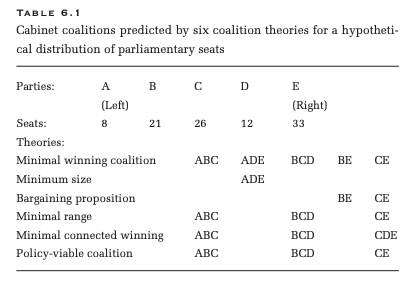
\includegraphics[width = 10cm]{fig 6.1.jpg}
                \end{center}
                \item Many theories tend to point back to a MWC framework; Lijphart sees this as oversimplifying and ignoring evidence of oversized (and minority) coalitions
                \item Strong negative correlation between effective number of parties and the percentage of either MWC or single-party cabinets (this may be tautological though?)
                \item Previous literature often uses cabinet durability as a metric of executive dominance; Lijphart agrees that it can be considered in part but disagrees that it should be used as a primary metric alone
                \item Strong positive relationship between executive dominance and the percentage of cabinets which are either MWC or one-party
            \end{itemize}
            \item \underline{\# of parties (2 vs. many)}
            \item \underline{Majoritarian versus proportional representation}
            \begin{itemize}
                \item Implied district threshold: $T = \frac{75}{M + 1}$ where $M$ is the average district magnitude
            \end{itemize}
            \item \underline{Pluralist interests versus ``corporatist'' centralized interest group systems}
        \end{enumerate}
        \item Federal-unitary dimension
        \begin{enumerate}
            \item \underline{Unitary (centralized) versus federal (decentralized)}
            \item \underline{Unicameral versus bicameral legislature}
            \item \underline{Flexibility of constitutions (accessibility of amendments)}
            \item \underline{Presence/absence of judicial review}
            \item \underline{(In)dependency of central banks from the executive}
        \end{enumerate}
        Primary possible explanation of clustering within these dimensions: Goodin (1996)'s distinction of ``collective agency \& shared responsibility'' with divided agencies and responsibilities
    \end{itemize}
    \item Central focus on the ``Westminster'' Model, equated to the majoritarian framework (and particularly that model within the United Kingdom). Defined by dominance of a usually single-party cabinet ruling with a very slight majority over a primary opposition party, elected by a majoritarian system. Unitary governmental system with a unicameral legislature. Broad constitutional flexibility (lack of a centralized UK constitution) with no judicial review, and a politically-dependent central bank.
    \item 
\end{itemize}


\section{Important Specific Factual Claims}

\begin{itemize}[leftmargin=*, itemsep=4pt]
    \item Relative internal homogeneity can reduce the downside of majoritarianism: even though exclusion from the ruling regime may not prove representative to the minority, if their interests are quite similar to those in the majority, then presumably the policy outcomes should be relatively congruent regardless. That is, even though government \emph{by} the people doesn't hold, government \emph{for} the people does.
\end{itemize}


\section{Connections}

\begin{itemize}
    \item Main findings from preceding book \emph{Democracies} (1984):
    \begin{enumerate}
        \item Democratic institutions can be measured on a scale from majoritarianism to consensus
        \item These two institutional structures form two clusters
        \item A 2-D conceptual map of democracy can be used to place these democracies
    \end{enumerate}
    \item References Huntington 1991 in suggesting a ``two-turnover test'': that a government can be recognized as a stable and consolidated democracy once a leadership transition $A \to B \to A$ occurs (not only can the opposition gain power, but they can also cede it back). Also uses Huntington's 1991 characterization of the three waves of democratization to identify eligible states
    \item Lewis (1965) argument of the incompatability of majoritarianism with democracy: ``to exclude the losing groups from participation in decision-making clearly violates the primary meaning of democracy.''
    \item Directly uses Dahl's polyarchy as a means of defining democracy and therefore selecting qualifying regimes
    \item \textcolor{red}{Primary difference from Powell is that Lijphart explicitly supports consensus democracy over majoritarianism: claims evidence shows that economic performance is not sacrified, but various other metrics of institutional success are enhanced under a proportional system}
    \item Boix 1999 uses Effective Electoral Threshold, similar methodological framework for measuring the ability of any party to gain meaningful representation
\end{itemize}


\section{My Critiques}

\begin{itemize}
    \item Opposition to MWC seems a bit contrived -- even though there are individual examples of oversized majorities, these are usually the case precisely because the conditions which drive MWC outcomes have not \emph{yet} come into effect. Namely, there is a high chance for collapse or consolidation later; that is, Lijphart is identifying outcomes, but not equilibrium outcomes.'
    \item Falls pretty bluntly within the comparative instinct to over-categorize... Created eight possible arrangements of legislative/executive tradeoffs and only three had any states (one of which only had one)
    \item Direction of causation in many of these relationships is unclear: does an increase in number of dimensions cause an increase in the number of parties, or vice versa? It is pretty clear that these can't be exclusively determined by the information given, but Lijphart seems to make some directional implications that are not necessarily substantiated in any meaningful sense
\end{itemize}


\end{document}
